\documentclass[12pt,fleqn]{article}\usepackage{../../common}
\begin{document}
Zaman Serilerini Sadece Evrisim ile Modelleme, Wavenet 

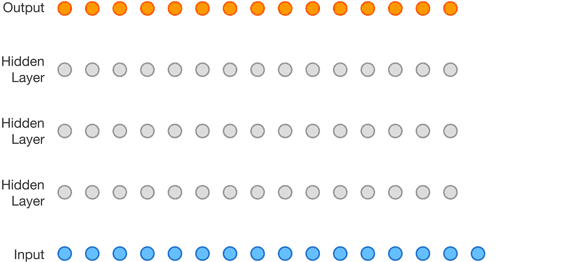
\includegraphics[width=20em]{wave-000.png}
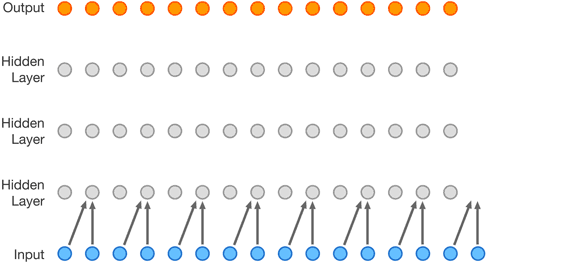
\includegraphics[width=20em]{wave-010.png}

\vspace{3em}

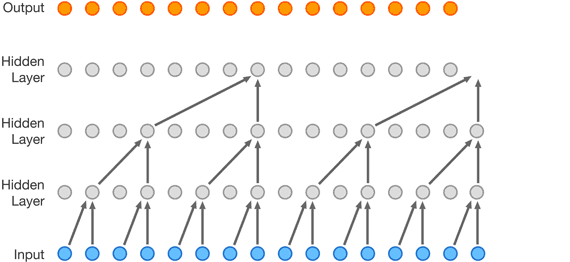
\includegraphics[width=20em]{wave-040.png}
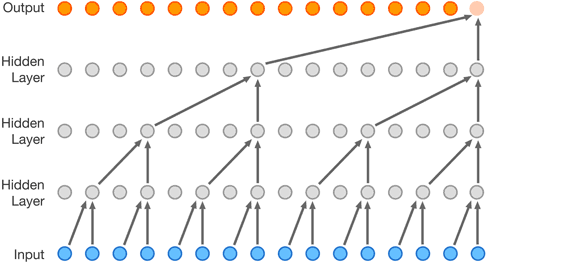
\includegraphics[width=20em]{wave-058.png}

\vspace{3em}

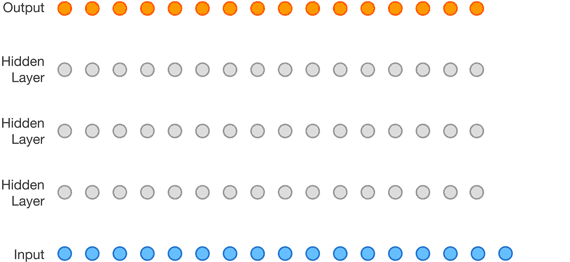
\includegraphics[width=20em]{wave-089.png}
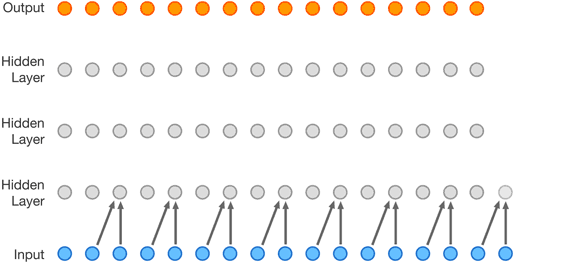
\includegraphics[width=20em]{wave-104.png}

\vspace{3em}

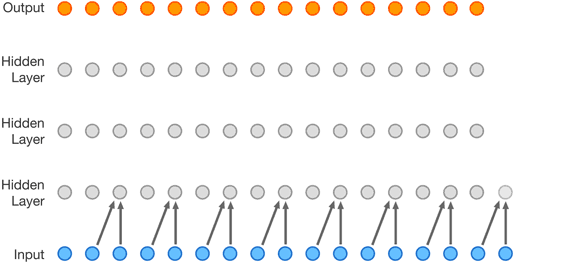
\includegraphics[width=20em]{wave-104.png}
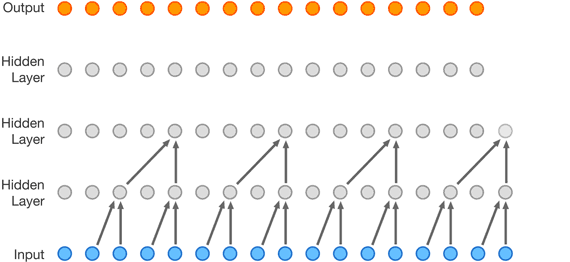
\includegraphics[width=20em]{wave-119.png}

\vspace{3em}

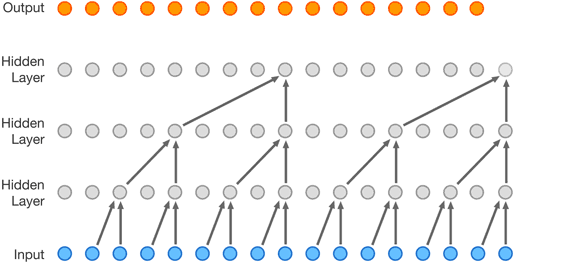
\includegraphics[width=20em]{wave-134.png}
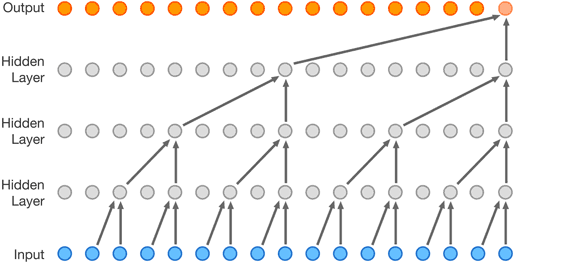
\includegraphics[width=20em]{wave-149.png}

\vspace{3em}

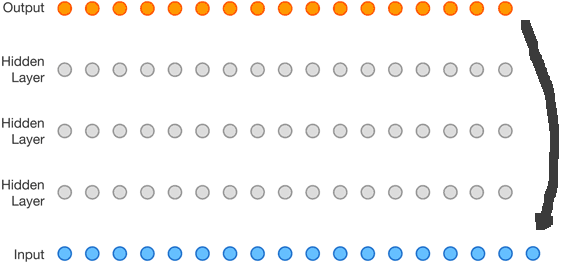
\includegraphics[width=20em]{wave-179.png}









\url{https://bair.berkeley.edu/blog/2018/08/06/recurrent/}

\url{https://github.com/JEddy92/TimeSeries_Seq2Seq/blob/master/notebooks/TS_Seq2Seq_Intro.ipynb}

\url{https://jeddy92.github.io/JEddy92.github.io/ts_seq2seq_conv}

\url{https://github.com/philipperemy/keras-tcn}

\url{https://arxiv.org/pdf/1803.01271.pdf}

\url{https://github.com/locuslab/TCN}

\url{https://github.com/philipperemy/keras-tcn/blob/master/tcn/tcn.py}


\end{document}













